% C086 accurate equality case: a=1,c=3,e=3,lambda=2; F1=-3,A=1,F2=3.
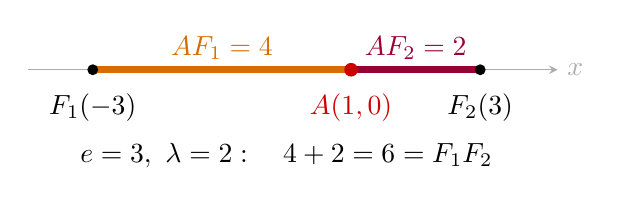
\begin{tikzpicture}[scale=0.82,>=stealth]
  \draw[->,gray!65] (-4.0,0)--(4.2,0) node[right] {$x$};
  \coordinate (Fone) at (-3,0);
  \coordinate (A) at (1,0);
  \coordinate (Ftwo) at (3,0);
  \draw[orange!85!black,line width=2.6pt] (Fone)--(A);
  \draw[purple!80!black,line width=2.6pt] (A)--(Ftwo);
  \fill (Fone) circle (2.4pt) node[below=5pt] {$F_1(-3)$};
  \fill[red!80!black] (A) circle (3pt) node[below=5pt] {$A(1,0)$};
  \fill (Ftwo) circle (2.4pt) node[below=5pt] {$F_2(3)$};
  \node[orange!85!black,above] at (-1,0) {$AF_1=4$};
  \node[purple!80!black,above] at (2,0) {$AF_2=2$};
  \node[below=23pt] at (0,0) {$e=3,\ \lambda=2:\quad 4+2=6=F_1F_2$};
\end{tikzpicture}
